\documentclass{article}
\usepackage{graphicx} % Required for inserting images
\graphicspath{ {./Images/} }
\usepackage{stackengine,scalerel}
\usepackage{enumitem}
\usepackage[utf8]{inputenc}
\usepackage{bm}
\usepackage{amsmath}
% \usepackage{amsmath}
\usepackage{mathtools}% Loads amsmath
\usepackage{amssymb}
\usepackage{listings}
\usepackage{multicol}
\usepackage{indentfirst}
\usepackage{hyperref}
\usepackage{xcolor}
%\setlength\parindent{0pt}
\allowdisplaybreaks
\usepackage{geometry}
 \geometry{
 a4paper,
 total={170mm,257mm},
 left=14mm,
 top=15mm,
 }
\setlength{\parindent}{0pt}
\title{MATH3205 - Paper Review}
\author{Hugo Burton, Anna Henderson and Mitchell Holt}
\date{August 2023}

\begin{document}

\maketitle

\section{Paper Review}

\subsection{Group Members}
Anna Henderson, Hugo Burton and Mitchell Holt

\subsection{Chosen Paper}
Title: Exact and metaheuristic methods for a real-world examination timetabling problem
Journal of Scheduling
\url{https://link.springer.com/article/10.1007/s10951-023-00778-6}


\subsection{Brief description of the problem that was solved}

The paper proposes the problem or organising Italian university exams in a given time horizon as well as allocating 0, 1 or multiple rooms for each exam. Courses are composite meaning exams can occur in multiple periods and/or multiple rooms. As the enrollment figures are not known at the time of planning, courses are grouped into curricula which determines which courses conflict and therefore need separation. The time horizon is divided into days with each day equally split into timeslots.

% The (hard) constraints are given explicitly:
% \begin{enumerate}[label=H\arabic*]
%     \item \emph{RoomRequest}. rooms assigned must be the correct size and quantity
%     \item \emph{RoomOccupation}. There must be at most one event per room per period
%     \item \emph{HardConflicts}. if they are both primary courses of one curriculum or have the same teacher.
%     \item \emph{Precedences}. if one even precedes another then the first must be scheduled before the other. E.g they are written and oral parts of the same curriculum or they are part of two consecutive exams of the same course
%     \item \emph{Unavailabilities}. Events cannot be assigned to an unavailable period or room
% \end{enumerate}

% \bigbreak

% The objective value is a weighted sum of the \emph{soft constraints} violated, which are:

% \begin{enumerate}[label=S\arabic*]
%     \item \emph{SoftConflicts}. Two events should have different periods if they are in soft conflict i.e. belong to courses that are in the same curriculum either as primary or secondary or both as secondary.
%     \item \emph{Preferences}. Events should not be assigned to an
%     undesired period or an undesired room. A period can also
%     be specified as preferred (a positive preference), so that in
%     case of preferred periods for an event, all indifferent ones
%     are assumed undesired (and explicitly undesired one are
%     given a larger penalty).
%     \item \emph{Distances}. Requested period separations between
%     events should be observed. We have two types of separations: directed, the first event must precede the second
%     one, and undirected.
% \end{enumerate}

\bigbreak
    
\subsection{Brief description of the solution technique used in the paper}

Two MIP formulations were proposed in the paper: a direct formulation and a two-stage problem where exams were first allocated to time periods and then rooms were allocated to exams. The paper found that the two-stage implementation was significantly faster, but it is not guaranteed that a time allocation in the first stage will admit a feasible solution in the second stage. \medbreak

Moreover, the two-stage model does not guarantee that any solution is feasible with respect to allocating composite rooms in the second stage | the model only considers composite room conflicts for composite rooms with the same number of member rooms. On all of the data instances the model was run against, no solutions were found to be infeasible, but the two-stage decomposition is nonetheless not as robust as the direct integer formulation.

\bigbreak

\subsection{What ideas, if any, you have for improving the solution technique}

One idea is to split the problem using Benders Decomposition, where the master problem would leave out some of the hard/soft constraints of the global problem - i.e. determine the time slot allocation of exams. The sub-problem would then be the room allocation and remaining constraints given the constraints imposed by the master problem. \\
\\
\noindent The paper notices that the capacities for composite rooms is the independence number of the conflict graph. We could construct these graphs in each time period to check (in callback) for composite room member conflicts. An example from the paper is five single small rooms $(\{A, B, C, D, E\})$ can be allocated to three $(2, S)$ $(\{AB, BC, C D\})$ and two $(3, S)$ $(\{ABC, C D E\})$ composite rooms. By inspection of the conflict graph (below), we may see that at most two of the $(2, S)$ or one of the $(3, S)$ can be used at one time, although the two-stage formulation proposed in the paper would not notice this:
\begin{center}
    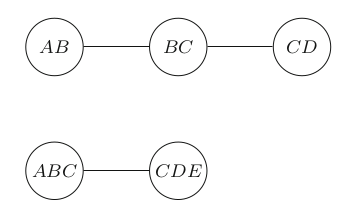
\includegraphics[scale=0.5]{graph.png}
\end{center}

\subsection{Where you are going to get data}

Data is linked in the paper at \url{https://bitbucket.org/satt/examtimetablinguniuddata} \medbreak

The Bitbucket has many instances of individual problem sets - some large and some small which we can use to test our model. Additionally, the solutions to each of these problem sets are provided. Both are in JSON format which we can read into Python very easily.

\bigbreak

\subsection{Preferred day for presenting (Wednesday or Thursday)}

We would prefer Wednesday but are all available either day.

\end{document}
